\subsubsection{Optimisation and Fitting}

The optimiser finds the model parameters that best fit the model to the current background subtracted video frame. Figure~\ref{fig:modelfit} shows the objective of the optimiser.

\begin{figure}[H]
    \centering
    \subfigure[Background Subtracted Frame]{
            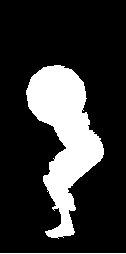
\includegraphics[height= 7cm]{algorithm/images/modelmatchbg}
    }
    \subfigure[Model]{
            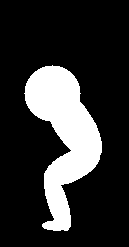
\includegraphics[height= 7cm]{algorithm/images/modelmatch}
    }
\caption{The model (b) is fit to the background subtracted frame (a)}
\label{fig:modelfit}
\end{figure}

The optimiser does this using an optimisation algorithm and a cost function.

The optimisation algorithm used is BOBYQA, which stands for Bound Optimisation BY Quadratic Approximation. This is an iterative algorithm for finding the minimum value of a function, given a set of bounded variables. The algorithm was developed by M. Powell, and is detailed in his paper\cite{bobyqa}.

The main advantages over other multivariate optimisation algorithms are firstly that it does not require derivatives of the cost function, and secondly that it constrains the search space using bounds. With no requirement for derivatives, the cost function can be treated as a `black box', allowing for far more freedom in the design of the cost function. In the case of this project, the cost function will need to perform operations on the model and video frames, and so is not a straightforward function of the input variables. The bounds reduce the search space which speeds up the time taken to find the parameters that best fit the model to the frame. With the right bounds, the chance of the model fitting to the frame in a position that is humanly impossible is reduced.

Another optimisation algorithm that could have been used is the widely known Nelder-Mead method\cite{neldermead}. Whilst Nelder-Mead is also a derivative-free optimisation method, it does not have the advantage of bounds. Bounds could be introduced in the cost function itself, but this would lead to a less predictable cost function, and therefore a more difficult function to minimise. Nelder-Mead is also a slower optimisation method, and performance is a critical factor in this application due to the goal of real-time tracking and analysis. The Apache Commons Math library\cite{apachemath} provides a Nelder-Mead optimisation method, which was trialled for this project but deemed too CPU intensive for real-time processing.

The application uses a Java implementation of BOBYQA, also available in the Apache Commons Math library\cite{apachemath}. One of the parameters it takes the set of bounds, which are input as a set of minimum and maximum angles for each joint in the model. These were chosen to give a generous range of motion for a squat, whilst restricting angles that would be humanly impossible to achieve.

For this application, the speed of the fitting also affects the quality of the fitting. The overall fit across multiple frames is affected both by the quality of the fit to each individual frame, and the number of frames fit to. As the speed of the optimisation in an individual frame increases, the number of frames we are able to fit to also increases. Likewise, as the speed of the optimisation in an individual frame decreases, we are able to fit to less frames in a given time period.

The main BOBYQA parameter that directly affects both the quality and speed of fitting to an individual frame is the number of `interpolation points'. The accuracy and performance trade-off is described in the BOBYQA paper\cite{bobyqa}. In the paper, a value of $2n + 1$, where $n$ is the number of cost function variables (ie. the number of degrees of freedom of the model) is stated as most commonly used to give a good balance of performance and accuracy. However in practice in this application it caused the frame rate to drop, and the overall fit over multiple frames to become less accurate. Trialling different values, it was determined that the optimal value was the minimum permitted number of interpolation points, $n + 2$. This maximised the frame throughput, and although the fit was less accurate per-frame, the increased number of frames that could be optimised over gave a better overall fit.

During the development of the tracking algorithm, a few different cost functions were evaluated before settling on the final implementation.

The first cost function attempt was one that returns the sum of squared distance from each joint in the model to the silhouette of the figure in the frame. The idea behind this was that by minimising these distances, the model's `skeleton' would always remain within the figure's silhouette. This function performed quite poorly, with the model roughly gravitating towards the silhouette, but never fitting properly.

The second cost function attempt was one that calculates the number of overlapping pixels when drawing the model directly on top of the silhouette. The number of pixels that overlap are to be maximised, and so we minimise the number of pixels of background that are not included in the overlap. Overlap $o$ is maximised by minimising $(w * h) - o$, where $w$ and $h$ are the width and height of the frame respectively. Overlap is calculated by performing a bitwise AND operation on the binary silhouette frame $f$ with a binary frame on which the model has been drawn $m$. This gives a binary frame where values are 1 for pixels that overlap, and 0 for pixels that do not. The number of non-zero pixels are counted to give the overlap value $o$. This gives the cost function:

\centerline{$cost = (w * h) - countNonZero(m \& f)$}

The third attempt was to minimise pixels of the model that did not overlap the silhouette, giving a cost function:

\centerline{$cost = countNonZero(m \& ~f)$}

The second cost function seemed to provide the best fit, and it is likely that this is due to the larger cost value returned by the second function being less likely to change dramatically for small changes in the model angles. For this reason the second cost function was chosen for the algorithm.

Figure~\ref{fig:modeloverlap} shows the model drawn on top of the foreground frame. Pixels coloured white are those that overlap after running BOBYQA using the chosen cost function. Pixels in grey are those of the model and foreground that do not overlap. Thus the chosen cost function attempts to minimise the number of grey and black pixels.

\begin{figure}[H]
    \centering
    \subfigure{
            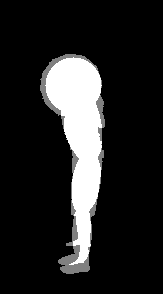
\includegraphics[height= 7cm]{algorithm/images/modelfitstart}
    }
    \subfigure{
            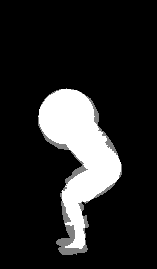
\includegraphics[height= 7cm]{algorithm/images/modelfitmid}
    }
    \subfigure{
            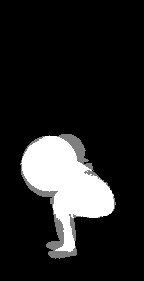
\includegraphics[height= 7cm]{algorithm/images/modelfitend}
    }
\caption{Model fitting by minimising pixels that do not overlap}
\label{fig:modeloverlap}
\end{figure}

At this stage in the algorithm we have obtained a foreground frame and a model, and through the optimisation the model has been fit to the foreground. Therefore on each frame the model is in the same position as the figure performing the squat. This does assume that the fit was perfect, which in practice is not the case, but the fit is generally good enough to assume that the model is in a position reasonably similar to that of the figure.